\documentclass[12pt, letterpaper]{article}
\usepackage[spanish]{babel}
\usepackage[utf8]{inputenc}
\usepackage{graphicx}
\usepackage{amssymb}
\graphicspath{{./imagenes/}}
\usepackage{xcolor}

%Paquetes para símbolos y entornos matematicos. En este documento se usa para poder usar el tag \begin{align} y \begin{align*} que permiten alinear expresiones matemáticas
\usepackage{amsmath}
\usepackage{amssymb}
%paquete que permite el uso de del argumento H al momento de insertar imágenes
\usepackage{float}

%comando para especificar el título del documento 
\title{Matemáticas para las Ciencias Aplicadas I}

%comando para especificar el autor del documento
\author{Pérez Romero Natalia Abigail}

%comando para especificar la fecha del documento
\date{\today}
%--------------Fin preámbulo--------------

%------------Inicio documento-------------
\begin{document}
%comando que genera el titulo con los datos especificados en el preámbulo
\maketitle
\textbf{Tarea VI. Ejercicios del libro Cálculo. Una variable de Thomas J.R, George B.}

\textbf{Ejercicios 2, 11 ,18 , 52 y 53 de la sección 1.5}

\textbf{Encuentre el dominio y el rango de $f, g, f+g,$ y $f * g$ }

 %sección 1.5 Combinación de Funciones del Thomas y me hacen los ejercicios 2, 11, 18, 52 y 53 de la sección.

(2) $f(x) = \sqrt{x+1}$, $g(x)= \sqrt{x-1}$

\begin{align*}
	x+1  \geq 0\\
	x \geq -1\\
	\therefore Dom(f) = [-1, \infty)
\end{align*}

\begin{align*}
	f(x) = \sqrt{x+1}\\
	 y = \sqrt{x+1}\\
	y^2 = {\sqrt{x+1}}^2\\
	y^2 = x+1\\
	y^2 -x = 1\\
	-x = 1- y^2\\
	x = -1+ y^2\\
	\therefore Im(f) = \mathbb{R}+, Im(f) = [0, \infty)
\end{align*}

\begin{figure}[h]
\centering
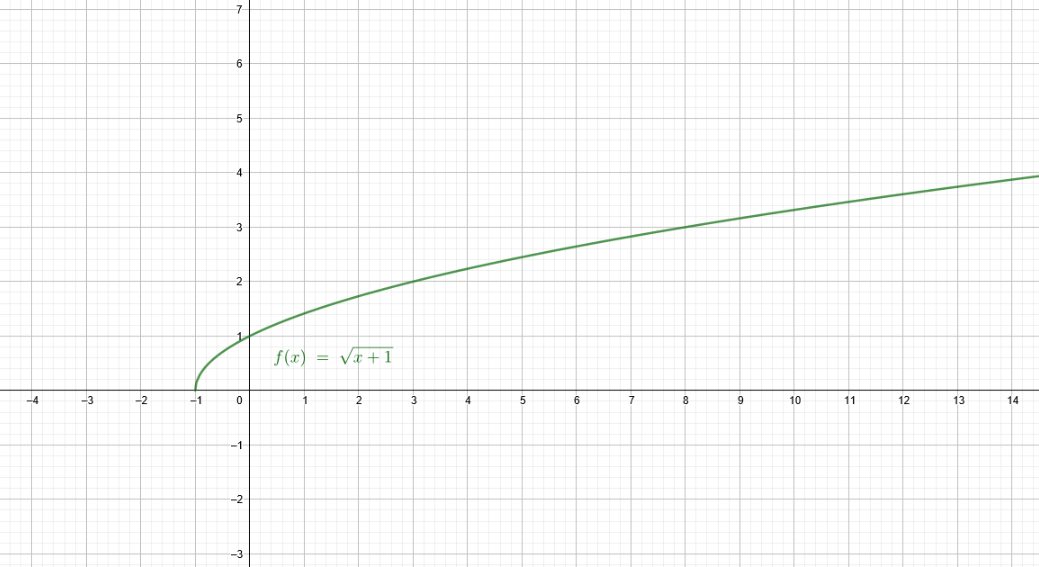
\includegraphics[width=30em]{t6uno}
\end{figure}

\newpage

\begin{align*}
	x-1  \geq 0\\
	x \geq 1\\
	\therefore Dom(g) = [1, \infty)
\end{align*}

\begin{align*}
	g(x)= \sqrt{x-1}
	y^2 = {\sqrt{x-1}}^2\\
	y^2 = x-1\\
	-x+y^2 = -1\\
	-x= -1- y^2\\
	 x= 1+ y^2\\
	\therefore Im(g) = \mathbb{R}+, Im(g) = [0, \infty)
\end{align*}

\begin{figure}[h]
\centering
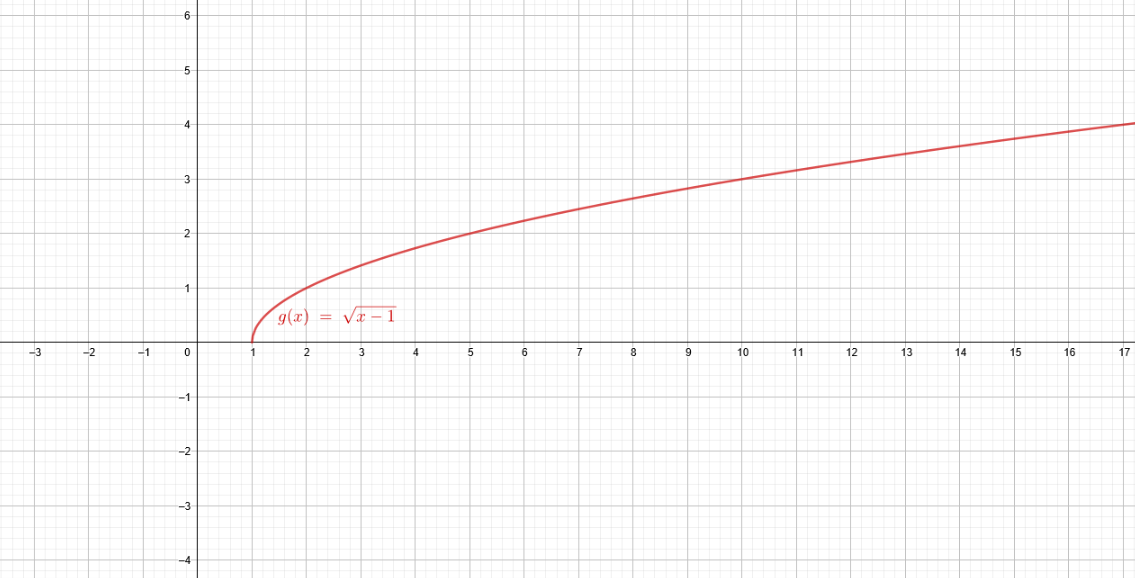
\includegraphics[width=30em]{t6dos}
\end{figure}

\textbf{$f+g(x) = f(x) + g(x)$}

\begin{align*}
	f+g(x) = \sqrt{x+1} + \sqrt{x-1}\\
	h(x) = \sqrt{x+1} + \sqrt{x-1}\\
	x + 1 \geq 0\\
	x \geq -1\\
	x  \geq 1
\end{align*}
De esta manera obtenemos lo intervalos $(-\infty, -1), (-1,1) , (1, \infty)$ 

Se evalua $(-\infty, -1)$ tomando un valor de este intervalo $x = -2$
	
\begin{align*}
	 \sqrt{(-2)+1} + \sqrt{(-2)-1} = 
	 \sqrt{-1} + \sqrt{-3}
\end{align*}
Como obtengo raíces negativas este intervalo no es valido

Se evalua $(1, \infty)$ tomando un valor de este intervalo $x = 2$
\begin{align*}
	 \sqrt{(2)+1} + \sqrt{(2)-1} = 
	 \sqrt{3} + \sqrt{1} = \sqrt{3} + 1
\end{align*}

He obtenido valores reales 	$\therefore Dom(f+g(x)) = (1, \infty)$

Por definicion el dominio de $f+g(x) = f(x) + g(x)$ es $D(f) \cap D(g)$
Dado $Dom(g) = [1, \infty)$ y $Dom(f) = [-1, \infty)$


\begin{align*}	
	[-1, \infty) \cap [1, \infty)\\
	Dom(f+g(x)) = (1, \infty)\\
	Im(f+g(x)) = \mathbb{R}+, Im(g) = [0, \infty) 
\end{align*}

\begin{figure}[h]
\centering
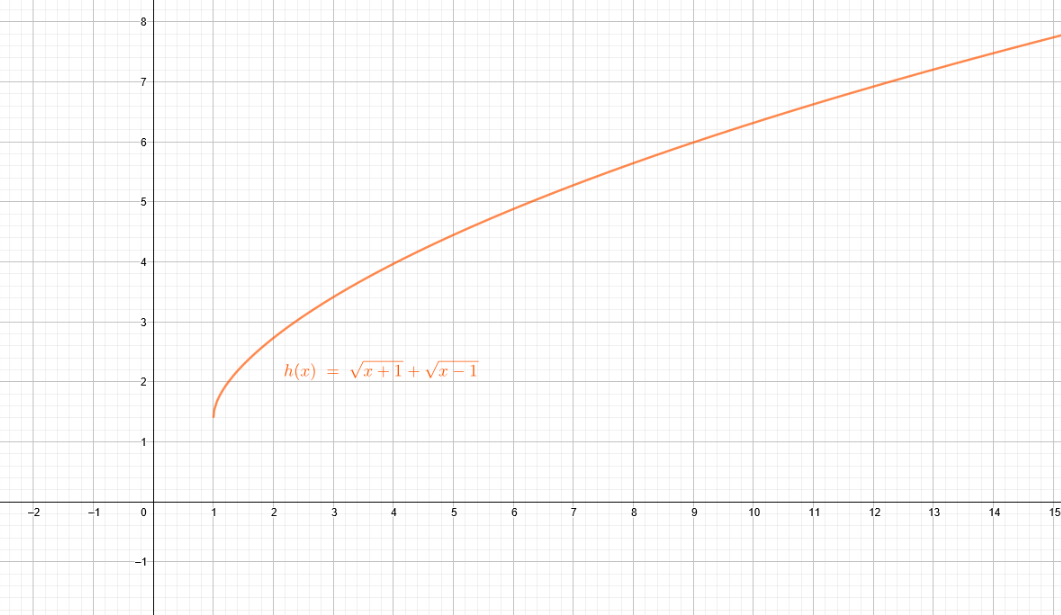
\includegraphics[width=30em]{t6tres}
\end{figure}

\newpage
\textbf{$(fg)(x)=f (x)* g(x)$}

\begin{align*}
	(fg)(x) = \sqrt{x+1} * \sqrt{x-1}\\
	p(x) = \sqrt{(x+1)(x-1)}\\
	p(x) = \sqrt{(x^2-1)}\\
	x^2-1 \geq 0\\
	x^2\geq 1\\
	x \geq \pm\sqrt{1}\\
	x  = -1\\
	x  = 1
\end{align*}

De esta manera obtenemos lo intervalos $(-\infty, -1), (-1,1) , (1, \infty)$ 

Se evalua $(-\infty, -1)$ tomando un valor de este intervalo $x = -2$
\begin{align*}
	\sqrt{(-2)^2-1}=\\
	\sqrt{4 - 1} = \sqrt{3}\\
\end{align*}
He obtenido valores reales 

Se evalua $(-1,1)$ tomando un valor de este intervalo $x = 0$
\begin{align*}
	\sqrt{(0)^2-1}=\\
	\sqrt{-1}\\
\end{align*}
Como obtengo raíces negativas este intervalo no es valido 

Se evalua $(1, \infty)$ tomando un valor de este intervalo $x = 2$
\begin{align*}
	\sqrt{(2)^2-1}=\\
	\sqrt{4 - 1} = \sqrt{3}\\
\end{align*}
He obtenido valores reales 

$\therefore Dom(p) = (-\infty, -1) \cup (1, \infty)$

\begin{figure}[h]
\centering
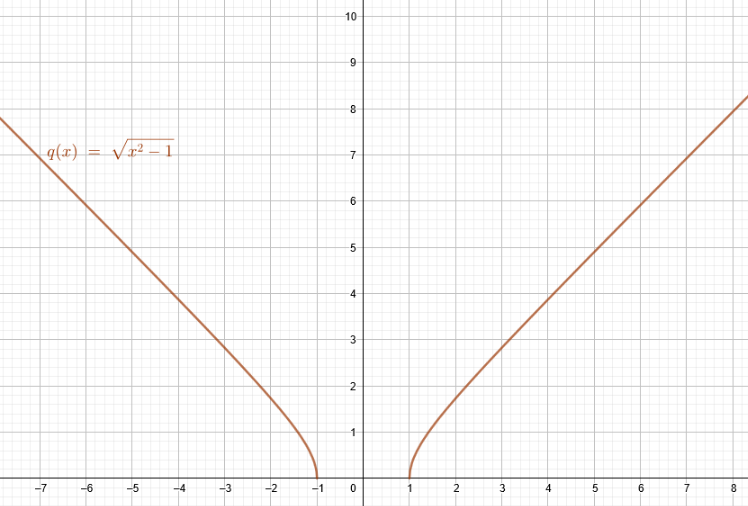
\includegraphics[width=30em]{t6cuatro}
\end{figure}

Sin embargo, por definicion el dominio de $(fg)(x)=f (x)* g(x)$ es $D(f) \cap D(g)$
Dado $Dom(g) = [1, \infty)$ y $Dom(f) = [-1, \infty)$


\begin{figure}[h]
\centering
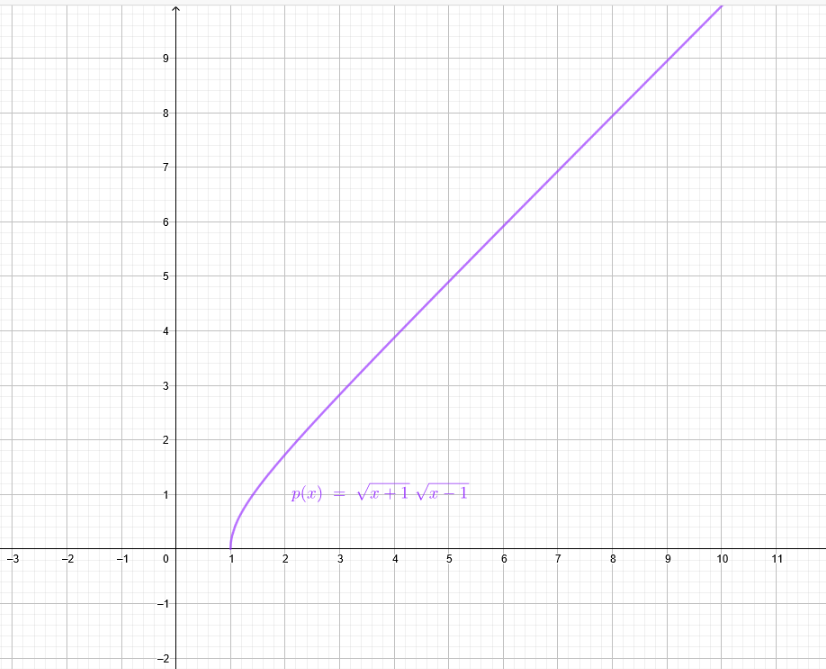
\includegraphics[width=30em]{t6cinco}
\end{figure}

\begin{align*}	
	[-1, \infty) \cap [1, \infty)\\
	Dom((fg)(x)) = (1, \infty) \\
	Im((fg)(x)) = \mathbb{R}+, Im(g) = [0, \infty)
\end{align*}

(11) Copie y complete la tabla siguiente:

\begin{tabular}{c c c c}
   &g(x) & $f(x)$ & $(f \circ g)(x) = f(g(x))$\\
\hline
a  & $x-7$                        & $\sqrt{x}$          & \textcolor{blue}{$f(x-7) = \sqrt{x-7}$} \\
b. & $x+2$                       & $3x$                 & \textcolor{blue}{$f(x+2) = 3(x+2) = 3x+6$} \\
c. & \textcolor{blue}{$x^2$}   & $\sqrt{x-5}$        & $\sqrt{x^2 -5}$ \\
d. & $\frac{x}{x-1}$           & $\frac{x}{x-1}$  & \textcolor{blue}{$f(\frac{x}{x-1}) = \frac{(\frac{x}{x-1})}{(\frac{x}{x-1})-1} = \frac{\frac{x}{x-1}}{\frac{x}{x-1}-\frac{1}{1}} = \frac{\frac{x}{x-1}}{\frac{x-x-1}{x-1}} = \frac{\frac{x}{x-1}}{\frac{-1}{x-1}} = \frac{x^2-x}{x+1} = - \frac{x(x+1)}{x+1} = x$} \\

e. & \textcolor{blue}{$\frac{x}{x-1}$}   & $1+\frac{1}{x}$        & $x$ \\
d. & $\frac{1}{x}$              & \textcolor{blue}{$x^{-1}$} & $x$ 
\end{tabular}

$f(\frac{x}{x-1}) = \frac{(\frac{x}{x-1})+1}{(\frac{x}{x-1})} = \frac{\frac{x}{x-1}}{\frac{x}{x-1}}$

(18) La figura siguiente muestra la gráfica de $y = -x^2$ desplazada a cuatro posiciones nuevas. Determine la función para cada nueva gráfica

\begin{figure}[h]
\centering
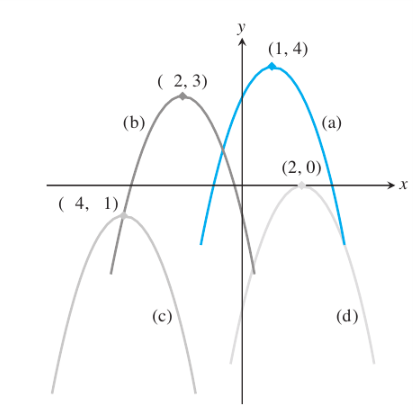
\includegraphics[width=25em]{graficaT5}
\end{figure}

\textbf{Encuentre una ecuación para cada gráfica estirada o comprimida}

(52) $y = x^2 -1$, comprimida horizontalmente por un factor de 2.

(53) $y = 1 + \frac{1}{x^2}$, comprimida verticalmente por un factor de 2.


\end{document}